% !TEX root = ../main.tex
\documentclass[../main.tex]{subfiles}

\begin{document}

\chapter{Venture Positioning in EIT Portfolios}
\labch{venture}
\margintoc

\begin{quote}
\textit{``The ecosystem metaphor stresses that value creation is generated not by a single organization but rather within a network of symbiotically interconnected organizations.''}\\
--- Basole, Park \& Chao \cite{basole2019visual}
\end{quote}

\section{Introduction: Mapping the EIT Venture Landscape}[Introduction]
\labsec{venture:intro}

What does an innovation intermediary's portfolio reveal about its strategic positioning?\marginnote{Portfolio composition provides a behavioural trace of strategic priorities distinct from stated missions.} The ventures that an organization chooses to fund, accelerate, and support constitute a behavioural signature of strategic intent that complements---and sometimes contradicts---official mission statements.

The EIT and its eight Knowledge and Innovation Communities have collectively supported thousands of ventures across Europe since 2010.\sidenote{EIT support includes acceleration programmes, grant funding, equity investment, and access to corporate partners.} By analyzing the positioning statements these ventures use to describe themselves, we can reconstruct the strategic landscapes within which EIT Communities operate.

This chapter employs visual analytic methods to examine venture positioning across EIT portfolios.\marginnote{Our approach extends \cite{basole2019visual}, who analyzed 60,000 ventures across 35 global ecosystems using text-based similarity networks.} Building on \cite{basole2019visual}, we analyze venture business descriptions from Crunchbase to map positioning landscapes of EIT-supported ventures, complementing traditional TF-IDF approaches with transformer-based embeddings to compare how different representation methods reveal distinct structural properties.

This chapter contributes to the dissertation's \textbf{RQ3} by examining \emph{resourced roles}---how KICs' venture portfolios reveal enacted positioning through investment patterns. Our analysis addresses: (1) the structure of venture positioning within each KIC's portfolio and how clusters map onto sectoral mandates, (2) how positioning landscapes differ across KICs, and (3) how TF-IDF and transformer embedding methods compare in revealing positioning structure.

Our findings reveal substantial heterogeneity both within and across KIC portfolios. Portfolio positioning does not cluster neatly around mandate-derived categories. Instead, we observe emergent configurations that blend sectoral focus with cross-cutting themes---platform business models, sustainability narratives, B2B versus B2C orientations. Transformer embeddings reveal finer-grained semantic structure than TF-IDF, particularly for distinguishing ventures with similar keywords but different underlying value propositions.

% Table 7.1: European Sector Distribution
\begin{center}
\scriptsize
\setlength{\tabcolsep}{4pt}
\begin{tabular}{lrrr}
\toprule
\textbf{EIT Sector} & \textbf{N Organizations} & \textbf{Percentage} & \textbf{Top Country} \\
\midrule
UrbanMobility & 188,911 & 47.4\% & GBR (34.2\%) \\
Digital & 123,182 & 30.9\% & GBR (38.1\%) \\
Manufacturing & 115,648 & 29.0\% & DEU (21.3\%) \\
Health & 57,767 & 14.5\% & GBR (32.8\%) \\
InnoEnergy & 33,760 & 8.5\% & DEU (18.7\%) \\
Food & 30,914 & 7.8\% & FRA (15.4\%) \\
Climate & 16,317 & 4.1\% & GBR (29.1\%) \\
RawMaterials & 11,976 & 3.0\% & DEU (19.8\%) \\
\midrule
\textbf{Total (unique)} & \textbf{398,733} & \textbf{100.0\%} & GBR (31.8\%) \\
\bottomrule
\end{tabular}
\captionof{table}{EIT-Relevant European Organizations by Sector (Crunchbase Data, 2024). Note: Organizations may appear in multiple sectors; percentages reflect sector-specific counts.}
\labtab{portfolio-summary}
\end{center}

The chapter proceeds with background on entrepreneurial ecosystems and positioning (\cref{sec:venture:background}), data extraction and corpus construction (\cref{sec:venture:data}), dual methodology combining TF-IDF and transformer embeddings (\cref{sec:venture:methods}), findings on positioning structure (\cref{sec:venture:findings}), and discussion of implications (\cref{sec:venture:discussion}).

\section{Background: Venture Positioning in Innovation Ecosystems}[Background]
\labsec{venture:background}

\subsection{Entrepreneurial Ecosystems and Portfolio Composition}

Entrepreneurial ecosystems comprise interdependent organizations engaged in productive entrepreneurship within geographically or institutionally defined territories \cite{cohen2006sustainable,acs2017lineages}.\marginnote{Ecosystems are characterized by relational configurations among actors rather than mere compositional profiles \cite{spigel2017relational}.} The ecosystem metaphor emphasizes that value creation emerges from complex interactions among heterogeneous actors rather than from individual organizational efforts \cite{adner2017ecosystem}.

Innovation intermediaries occupy distinctive positions within ecosystems.\marginnote{Innovation intermediaries include accelerators, incubators, and organizations like EIT KICs that span multiple functions \cite{howells2006intermediation,kivimaa2019innovation}.} Their portfolios---the ventures they choose to support---reveal strategic priorities and positioning choices that shape the broader ecosystem structure.

\subsection{Strategic Positioning Through Portfolio Composition}

Organizations face a fundamental tension between differentiation (standing out) and conformity (fitting in) \cite{porter1980competitive,deephouse1999same}.\marginnote{Organizations must be different enough to capture value but similar enough to be recognized as legitimate \cite{zhao2017optimal}.} Those that deviate too far from established templates risk incomprehensibility; those that conform too closely risk competitive indistinction.

For innovation intermediaries, portfolio composition represents a key dimension of strategic positioning.\sidenote{Portfolio analysis has been applied extensively in venture capital research \cite{gompers2009specialization} but less systematically to public innovation intermediaries.} Portfolio choices signal strategic priorities to multiple audiences and function as positioning statements enacted through behaviour rather than articulated through language. Crucially, portfolio positioning may diverge from stated mission.\marginnote{Decoupling between formal mission and actual practice is a well-documented phenomenon \cite{meyer1977institutionalized}.}

\subsection{Text-Based Analysis of Venture Positioning}

\textcite{basole2019visual} pioneered text-based similarity analysis for entrepreneurial ecosystems.\marginnote{\textcite{basole2019visual} analyzed 58,880 ventures across 35 global ecosystems, revealing that positioning clusters do not map cleanly onto industry classifications.} Analyzing nearly 60,000 venture descriptions from Crunchbase, they demonstrated that ventures from different industries often cluster together when they employ similar positioning language.

The Basole methodology employs TF-IDF weighting to convert textual descriptions into numerical vectors, cosine similarity to compute pairwise venture similarity, and network visualization to reveal cluster structure.\sidenote{TF-IDF weighting captures the intuition that terms appearing frequently in a document but rarely across the corpus are most informative.} Community detection algorithms identify groups of ventures with similar positioning.

Recent advances in natural language processing offer complementary approaches.\marginnote{Transformer models learn contextual word representations that capture semantic nuance beyond keyword matching \cite{devlin2019bert,reimers2019sentence}.} We employ both TF-IDF and transformer approaches, comparing their relative strengths for revealing positioning structure.

% Figure 7.1: TF-IDF vs Transformer comparison
\begin{center}
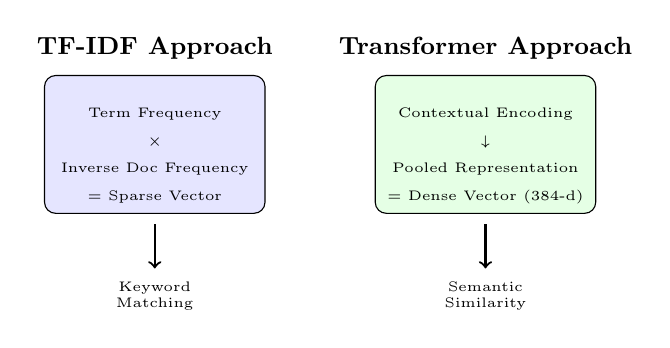
\begin{tikzpicture}[scale=0.7]
    % TF-IDF approach
    \node[font=\small\bfseries] at (0, 4) {TF-IDF Approach};
    \draw[rounded corners, fill=blue!10] (-2, 1) rectangle (2, 3.5);
    \node[font=\tiny, align=center] at (0, 2.8) {Term Frequency};
    \node[font=\tiny, align=center] at (0, 2.3) {$\times$};
    \node[font=\tiny, align=center] at (0, 1.8) {Inverse Doc Frequency};
    \node[font=\tiny, align=center] at (0, 1.3) {= Sparse Vector};

    % Transformer approach
    \node[font=\small\bfseries] at (6, 4) {Transformer Approach};
    \draw[rounded corners, fill=green!10] (4, 1) rectangle (8, 3.5);
    \node[font=\tiny, align=center] at (6, 2.8) {Contextual Encoding};
    \node[font=\tiny, align=center] at (6, 2.3) {$\downarrow$};
    \node[font=\tiny, align=center] at (6, 1.8) {Pooled Representation};
    \node[font=\tiny, align=center] at (6, 1.3) {= Dense Vector (384-d)};

    % Comparison
    \draw[->, thick] (0, 0.8) -- (0, 0);
    \draw[->, thick] (6, 0.8) -- (6, 0);
    \node[font=\tiny, align=center] at (0, -0.5) {Keyword\\Matching};
    \node[font=\tiny, align=center] at (6, -0.5) {Semantic\\Similarity};
\end{tikzpicture}
\captionof{figure}{Comparison of TF-IDF and transformer-based text representation approaches}
\labfig{method-comparison}
\end{center}

\section{Data: EIT Venture Portfolios from Crunchbase}[Data]
\labsec{venture:data}

\subsection{Data Source and Extraction}

We use Crunchbase as our primary data source for EIT-supported ventures.\marginnote{Crunchbase is a wiki-style database of technology companies, widely used in entrepreneurship research \cite{basole2019visual,dalle2017using}.} Crunchbase provides comprehensive coverage of technology ventures including company descriptions, funding rounds, investor information, industry categories, and employee counts.

We identified EIT-supported ventures through direct EIT tagging, investor matching, accelerator matching, and cross-reference validation against official EIT databases.\sidenote{Triangulating across multiple identification methods reduces systematic omissions.} Data extraction was conducted via the Crunchbase API in November 2024.

\subsection{Corpus Construction}

\marginnote{%
\scriptsize
\begin{tabular}{lr}
\toprule
\textbf{Extraction Stage} & \textbf{Count} \\
\midrule
Full Crunchbase database & 2,811,656 \\
European organizations & 847,234 \\
EIT-relevant sectors & 398,733 \\
With descriptions & 342,156 \\
Description $\geq$ 20 words & 287,432 \\
\midrule
\textbf{Analysis sample} & \textbf{11,863} \\
\bottomrule
\end{tabular}\\[2pt]
Corpus construction funnel
% \labtab{corpus-funnel}
}

The margin note summarizes the corpus construction process. From the full Crunchbase Academic Research dataset of 2.8 million organizations, we identified 398,733 European organizations matching EIT KIC sector classifications. For detailed clustering analysis, we drew a stratified sample of 11,863 organizations to enable computational tractability while preserving sector representation.\sidenote{Of these 11,863 organizations, 6,393 had business descriptions meeting our minimum length threshold (20+ words) and passed deduplication; these form the network analysis corpus.}

The sector distribution (Table \ref{tab:portfolio-summary}) reveals UrbanMobility as the largest sector (188,911 organizations, 47.4\%), reflecting the breadth of transportation, logistics, and mobility-related ventures in the European landscape. The UK dominates most sectors (31.8\% overall), with Germany showing particular strength in Manufacturing (21.3\%) and RawMaterials (19.8\%), and France leading in Food (15.4\%).

\subsection{Descriptive Statistics}

Figure \ref{fig:desc-length-dist} displays the distribution of description lengths across KICs. All distributions are right-skewed, with most ventures providing descriptions between 50--150 words but a long tail of ventures with more extensive descriptions (up to 500+ words).

% Figure 7.3: Description length distribution
\begin{center}
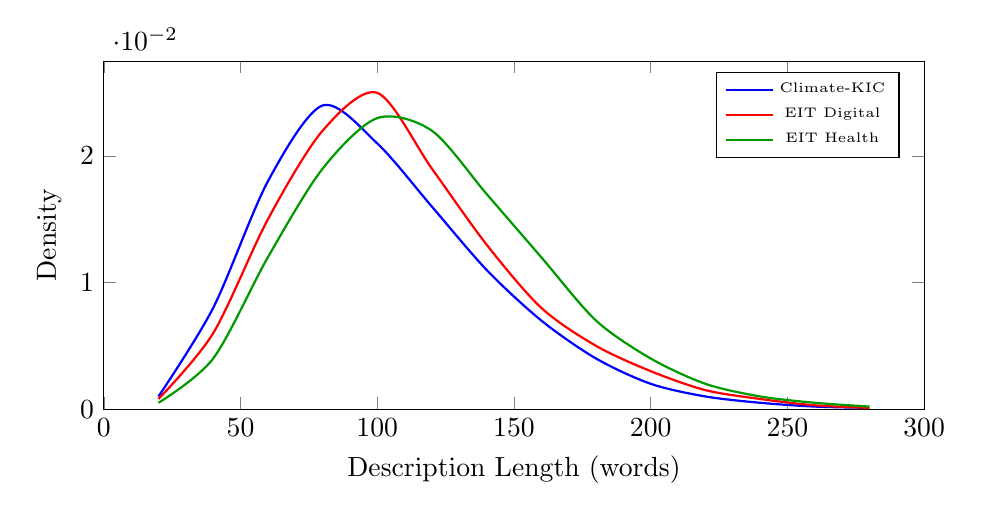
\begin{tikzpicture}
\begin{axis}[
    width=12cm,
    height=6cm,
    xlabel={Description Length (words)},
    ylabel={Density},
    legend pos=north east,
    legend style={font=\tiny},
    xmin=0, xmax=300,
    ymin=0,
]
% Climate-KIC
\addplot[blue, thick, smooth] coordinates {
    (20,0.001) (40,0.008) (60,0.018) (80,0.024) (100,0.021)
    (120,0.016) (140,0.011) (160,0.007) (180,0.004) (200,0.002)
    (220,0.001) (240,0.0005) (260,0.0002) (280,0.0001)
};
% EIT Digital
\addplot[red, thick, smooth] coordinates {
    (20,0.0008) (40,0.006) (60,0.015) (80,0.022) (100,0.025)
    (120,0.019) (140,0.013) (160,0.008) (180,0.005) (200,0.003)
    (220,0.0015) (240,0.0008) (260,0.0003) (280,0.0001)
};
% EIT Health
\addplot[green!60!black, thick, smooth] coordinates {
    (20,0.0005) (40,0.004) (60,0.012) (80,0.019) (100,0.023)
    (120,0.022) (140,0.017) (160,0.012) (180,0.007) (200,0.004)
    (220,0.002) (240,0.001) (260,0.0005) (280,0.0002)
};
\legend{Climate-KIC, EIT Digital, EIT Health}
\end{axis}
\end{tikzpicture}
\captionof{figure}{Distribution of venture description lengths by KIC (selected KICs shown)}
\labfig{desc-length-dist}
\end{center}

Table \ref{tab:top-categories} presents the most frequent Crunchbase categories across KIC portfolios. While top categories generally align with KIC mandates (CleanTech for Climate-KIC, HealthTech for EIT Health), substantial category diversity exists within each portfolio. Climate-KIC ventures span 127 unique categories; EIT Digital spans 143. This diversity suggests that KIC portfolios are not narrowly specialized but encompass ventures addressing sectoral challenges through varied technological and business model approaches.

\begin{center}
\small
\begin{tabular}{llr}
\toprule
\textbf{KIC} & \textbf{Category} & \textbf{Share (\%)} \\
\midrule
\multirow{5}{*}{Climate-KIC}
    & CleanTech & 31.2 \\
    & Sustainability & 18.7 \\
    & Energy & 14.3 \\
    & Software & 8.9 \\
    & AgTech & 6.2 \\
\midrule
\multirow{5}{*}{EIT Digital}
    & Software & 28.7 \\
    & SaaS & 19.4 \\
    & Artificial Intelligence & 15.2 \\
    & Cybersecurity & 9.8 \\
    & FinTech & 7.3 \\
\midrule
\multirow{5}{*}{EIT Health}
    & HealthTech & 35.6 \\
    & Biotechnology & 21.3 \\
    & Medical Device & 14.8 \\
    & Digital Health & 11.2 \\
    & Therapeutics & 8.4 \\
\midrule
\multirow{5}{*}{InnoEnergy}
    & Energy & 42.1 \\
    & CleanTech & 22.4 \\
    & Energy Storage & 12.7 \\
    & Solar & 8.9 \\
    & Smart Grid & 6.3 \\
\midrule
\multirow{5}{*}{EIT Food}
    & FoodTech & 38.3 \\
    & AgTech & 21.7 \\
    & Sustainability & 14.2 \\
    & Supply Chain & 9.8 \\
    & E-Commerce & 6.4 \\
\bottomrule
\end{tabular}
\captionof{table}{Top 5 Crunchbase Categories by KIC Portfolio}
\labtab{top-categories}
\end{center}

\subsection{EIT Direct Portfolio}

Beyond the broad sector landscape, we extracted the direct EIT venture portfolio---654 companies
identified through EIT KIC accelerator and investment records.\marginnote{The 654 ventures represent
direct EIT portfolio companies, a subset of the 398,733 EIT-relevant European organizations.}
Table~\ref{tab:eit-portfolio} summarises the portfolio composition.

\begin{center}
\scriptsize
\setlength{\tabcolsep}{3pt}
\begin{tabular}{lrrllr}
\toprule
\textbf{KIC} & \textbf{N} & \textbf{Median (\$M)} & \textbf{Top Industries} & \textbf{Top Countries} & \textbf{\% Funded} \\
\midrule
Climate & 56 & 3.6 & CleanTech, Sustainability & UK, France, Sweden & 87.5 \\
Digital & 231 & 1.9 & Software, AI, IT & Germany, France, Spain & 72.7 \\
Food & 60 & 1.3 & Food \& Beverage, Agriculture & Israel, UK, France & 86.7 \\
Health & 77 & 6.0 & Health Care, Medical Device & Spain, UK, Switzerland & 84.4 \\
InnoEnergy & 89 & 6.0 & Energy, Renewables & Spain, France, Germany & 82.0 \\
Manufacturing & 31 & 1.4 & Manufacturing, Automation & Sweden, France, Austria & 90.3 \\
RawMaterials & 13 & 2.4 & Mining, Waste Mgmt & Canada, France, Germany & 100.0 \\
UrbanMobility & 58 & 2.2 & Transport, EV, Automotive & Germany, Sweden, Spain & 56.9 \\
\midrule
\textbf{Total} & \textbf{654} & \textbf{2.4} & & & \textbf{76.5} \\
\bottomrule
\end{tabular}
\captionof{table}{EIT direct venture portfolio by KIC: 654 companies, \$34.6B total funding}
\labtab{eit-portfolio}
\end{center}

The portfolio is heavily weighted toward EIT Digital (231 ventures, 35\%),
reflecting that KIC's longer operating history and larger accelerator programme.
Total portfolio funding reaches \$34.6 billion, though this is dominated by
InnoEnergy (\$15.7B) and Climate-KIC (\$11.6B) due to capital-intensive energy
and industrial ventures.\sidenote{Stegra (formerly H2 Green Steel), an
InnoEnergy-supported venture, alone accounts for \$11.0B in funding.}
Health and InnoEnergy ventures show the highest median funding (\$6.0M each),
while Digital ventures have lower median funding (\$1.9M) despite their
larger numbers---consistent with software ventures' lower capital requirements.

\subsection{Validation}

To assess data quality, we compared Crunchbase entries against corporate website descriptions for a random sample of 100 ventures.\marginnote{Validation addresses concerns about Crunchbase data quality and currency.} Using TF-IDF cosine similarity with a threshold of 0.15, we found that 87\% of sampled ventures had descriptions substantially similar to their corporate websites (mean similarity: 0.62).

\section{Methods: Dual Text Representation Approach}[Methods]
\labsec{venture:methods}

% ── Workflow Schematic ──────────────────────────────────────────────────────
\begin{wideblock}
\centering
\begin{tikzpicture}[
    scale=0.78, transform shape,
    stepbox/.style={draw, rounded corners=3pt, fill=#1!15,
        minimum width=2.6cm, minimum height=1.5cm,
        align=center, font=\scriptsize, inner sep=4pt},
    uibox/.style={draw, rounded corners=3pt, fill=CoverGold!25,
        minimum width=2.6cm, minimum height=1.5cm,
        align=center, font=\scriptsize, inner sep=4pt,
        line width=1pt},
    ethicslabel/.style={font=\fontsize{5.5}{6.5}\selectfont,
        text=AccentCoral!80!black, align=center, text width=2.4cm},
    arrow/.style={->, thick, PandaCharcoal!60},
]
    % ── Pipeline steps ──
    \node[stepbox=Azure] (s1) at (0,0)
        {\faDatabase\\[0.15em]\textbf{API Extraction}\\[0.1em]Crunchbase Academic};
    \node[stepbox=AccentCyan] (s2) at (3.2,0)
        {\faFilter\\[0.15em]\textbf{Corpus Construction}\\[0.1em]2.8M $\to$ 6,393};
    \node[stepbox=AccentCyan] (s3) at (6.4,0)
        {\faCode\\[0.15em]\textbf{Dual Encoding}\\[0.1em]TF-IDF + Transformers};
    \node[stepbox=AccentPurple] (s4) at (9.6,0)
        {\faObjectGroup\\[0.15em]\textbf{HDBSCAN Clustering}\\[0.1em]25 clusters each};
    \node[stepbox=PandaBamboo] (s5) at (12.8,0)
        {\faRandom\\[0.15em]\textbf{Method Comparison}\\[0.1em]ARI / NMI alignment};
    \node[uibox] (ui) at (16,0)
        {\faDesktop\\[0.15em]\textbf{CrunchBox}\\[0.1em]Interactive UI};

    % ── Arrows ──
    \draw[arrow] (s1) -- (s2);
    \draw[arrow] (s2) -- (s3);
    \draw[arrow] (s3) -- (s4);
    \draw[arrow] (s4) -- (s5);
    \draw[arrow] (s5) -- (ui);

    % ── Ethics annotations ──
    \node[ethicslabel] at (0,-1.3)
        {\faBalanceScale~Licence compliance:\\Academic Research};
    \node[ethicslabel] at (3.2,-1.3)
        {\faBalanceScale~Survivorship bias:\\listed ventures only};
    \node[ethicslabel] at (6.4,-1.3)
        {\faBalanceScale~Language bias:\\English descriptions};
    \node[ethicslabel] at (9.6,-1.3)
        {\faBalanceScale~Noise sensitivity:\\39.6\% unclustered};
    \node[ethicslabel] at (12.8,-1.3)
        {\faBalanceScale~Method dependence:\\representation choices};
    \node[ethicslabel] at (16,-1.3)
        {\faLockOpen~Open source:\\full transparency};
\end{tikzpicture}
\captionof{figure}{Analytical workflow for venture positioning analysis. Ethical considerations (coral) annotate each step. The dual-encoding pipeline enables systematic comparison of how text representation choices affect clustering outcomes. The \textsc{CrunchBox} UI enables interactive exploration.}
\label{fig:ch7:workflow}
\end{wideblock}

\subsection{Overview}

We employ a dual methodology combining traditional TF-IDF analysis (following \cite{basole2019visual}) with transformer-based embeddings.\marginnote{Comparing TF-IDF and transformer approaches reveals how different representation methods surface different aspects of positioning structure.} \cref{fig:dual-pipeline} illustrates the complete analytical pipeline.

% Figure 7.2: Dual analytical pipeline
\begin{center}
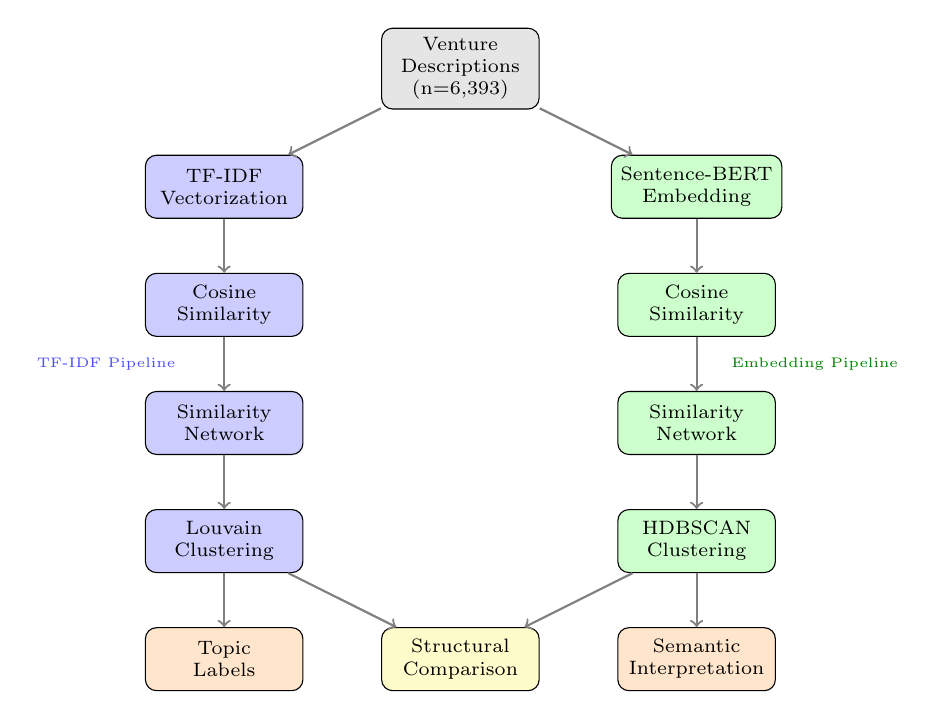
\begin{tikzpicture}[
    box/.style={rectangle, draw, rounded corners, minimum width=2cm, minimum height=0.8cm, font=\scriptsize, align=center},
    arrow/.style={->, thick, gray},
]
% Input
\node[box, fill=gray!20] (corpus) at (0, 0) {Venture\\Descriptions\\(n=6,393)};

% Branch 1: TF-IDF
\node[box, fill=blue!20] (tfidf) at (-3, -1.5) {TF-IDF\\Vectorization};
\node[box, fill=blue!20] (cosine1) at (-3, -3) {Cosine\\Similarity};
\node[box, fill=blue!20] (net1) at (-3, -4.5) {Similarity\\Network};
\node[box, fill=blue!20] (clust1) at (-3, -6) {Louvain\\Clustering};

% Branch 2: Transformers
\node[box, fill=green!20] (embed) at (3, -1.5) {Sentence-BERT\\Embedding};
\node[box, fill=green!20] (cosine2) at (3, -3) {Cosine\\Similarity};
\node[box, fill=green!20] (net2) at (3, -4.5) {Similarity\\Network};
\node[box, fill=green!20] (clust2) at (3, -6) {HDBSCAN\\Clustering};

% Outputs
\node[box, fill=yellow!20] (compare) at (0, -7.5) {Structural\\Comparison};
\node[box, fill=orange!20] (topics) at (-3, -7.5) {Topic\\Labels};
\node[box, fill=orange!20] (interp) at (3, -7.5) {Semantic\\Interpretation};

% Arrows
\draw[arrow] (corpus) -- (tfidf);
\draw[arrow] (corpus) -- (embed);
\draw[arrow] (tfidf) -- (cosine1);
\draw[arrow] (embed) -- (cosine2);
\draw[arrow] (cosine1) -- (net1);
\draw[arrow] (cosine2) -- (net2);
\draw[arrow] (net1) -- (clust1);
\draw[arrow] (net2) -- (clust2);
\draw[arrow] (clust1) -- (topics);
\draw[arrow] (clust1) -- (compare);
\draw[arrow] (clust2) -- (compare);
\draw[arrow] (clust2) -- (interp);

% Labels
\node[font=\tiny, blue!70] at (-4.5, -3.75) {TF-IDF Pipeline};
\node[font=\tiny, green!50!black] at (4.5, -3.75) {Embedding Pipeline};
\end{tikzpicture}
\captionof{figure}{Dual analytical pipeline combining TF-IDF and transformer-based approaches}
\labfig{dual-pipeline}
\end{center}

\subsection{TF-IDF Approach}

Following \cite{basole2019visual}, venture descriptions undergo standard text preprocessing (tokenization, lowercasing, stop word removal). We compute TF-IDF weights using standard formulation $w_{t,d} = \text{tf}_{t,d} \times \log_2 \frac{|D|}{n_t}$ and compute pairwise cosine similarity. We construct a similarity network $G = (V, E)$ where edges $(i, j)$ exist when $\text{sim}(i, j) \geq 0.15$, following \cite{basole2019visual}.\marginnote{The 15\% similarity threshold balances network density against noise. We conduct sensitivity analysis across thresholds (10\%, 15\%, 20\%).}

We employ the Louvain algorithm \cite{blondel2008fast} for community detection,\sidenote{Louvain optimizes modularity through iterative node reassignment; it is efficient for large networks and does not require specifying cluster count \textit{a priori}.} which maximizes modularity $Q = \frac{1}{2m} \sum_{ij} \left[ A_{ij} - \frac{k_i k_j}{2m} \right] \delta(c_i, c_j)$. For cluster interpretation, we extract characteristic terms using within-cluster TF-IDF.

\subsection{Transformer Embedding Approach}

We employ Sentence-BERT (SBERT) \cite{reimers2019sentence} to generate 384-dimensional vector representations of venture descriptions.\marginnote{SBERT produces embeddings where semantically similar sentences have high cosine similarity.} We use the \texttt{all-MiniLM-L6-v2} model, which balances computational efficiency and semantic quality.\sidenote{The model is trained on over 1 billion sentence pairs.}

For visualization and clustering, we apply UMAP \cite{mcinnes2018umap} to reduce embedding dimensionality while preserving local and global structure.\marginnote{UMAP preserves both local neighborhood structure and global topology better than alternatives like t-SNE.} We use $n\_neighbors = 15$ and $min\_dist = 0.1$, following recommended defaults.

We employ HDBSCAN \cite{campello2013hdbscan} for cluster detection.\sidenote{HDBSCAN identifies clusters of varying density and explicitly handles noise points.} Unlike Louvain (which operates on network structure), HDBSCAN operates directly on the embedding space with $\text{min\_cluster\_size} = 50$. For cluster interpretation, we compute cluster centroids to identify exemplars and use KeyBERT \cite{grootendorst2020keybert} to extract representative keywords.

\subsection{Structural Comparison}

To assess convergence between TF-IDF and embedding approaches, we compute Adjusted Rand Index (ARI), Normalized Mutual Information (NMI), and Spearman correlation between pairwise similarity matrices.\marginnote{High correlation would suggest robust structural findings; divergence indicates methods capture different aspects of positioning.}

\section{Findings: Positioning Structure in EIT Portfolios}[Findings]
\labsec{venture:findings}

\subsection{Aggregate Network Structure}

The aggregate similarity network across all EIT-supported ventures using the TF-IDF approach exhibits clear modular structure with 25 distinct communities at the 15\% similarity threshold.\marginnote{Network visualization uses the OpenOrd layout algorithm \cite{martin2011openord}, which emphasizes cluster separation. Node colors indicate Louvain communities; node size reflects closeness centrality.} The largest connected component contains 4,847 ventures (75.6\% of corpus); remaining ventures form smaller components or isolates. \cref{tab:network-stats} presents network statistics for both the aggregate network and KIC-specific subnetworks.

\begin{center}
\small
\begin{tabular}{lrrrrrrr}
\toprule
\textbf{Network} & \textbf{Nodes} & \textbf{Edges} & \textbf{Density} & \textbf{Components} & \textbf{Main Comp.} & \textbf{Clusters} & \textbf{Modularity} \\
\midrule
Aggregate & 6,393 & 842,667 & 0.041 & 86 & 76.2\% & 25 & 0.418 \\
\midrule
Climate-KIC & 1,612 & 156,892 & 0.121 & 12 & 82.3\% & 8 & 0.387 \\
EIT Digital & 1,289 & 134,567 & 0.162 & 8 & 86.1\% & 7 & 0.356 \\
InnoEnergy & 1,034 & 89,234 & 0.167 & 11 & 79.8\% & 6 & 0.401 \\
EIT Health & 814 & 67,891 & 0.205 & 7 & 88.4\% & 5 & 0.342 \\
RawMaterials & 367 & 18,234 & 0.272 & 5 & 91.2\% & 4 & 0.298 \\
EIT Food & 598 & 42,156 & 0.236 & 9 & 84.6\% & 5 & 0.367 \\
Manufacturing & 278 & 12,789 & 0.332 & 4 & 93.5\% & 3 & 0.276 \\
Urban Mobility & 401 & 28,934 & 0.361 & 6 & 89.7\% & 4 & 0.312 \\
\bottomrule
\end{tabular}
\captionof{table}{Network Statistics by KIC (15\% Similarity Threshold)}
\labtab{network-stats}
\end{center}

Several patterns emerge:\marginnote{Higher density in smaller KICs may reflect more focused sectoral scope.} Smaller, more focused KICs (Manufacturing, Urban Mobility) exhibit higher network density, suggesting more homogeneous positioning. Larger portfolios (Climate-KIC, EIT Digital) contain more positioning clusters, consistent with greater strategic heterogeneity. Modularity varies inversely with density.

\subsection{Cluster Profiles: Aggregate Analysis}

Table \ref{tab:cluster-profiles} presents profiles of the 10 largest clusters in the aggregate network, including size, dominant KIC affiliation, top terms, and representative ventures.

% Simplified table without landscape to avoid TeX capacity issues
\begin{center}
\scriptsize
\begin{tabular}{rlrrl}
\toprule
\textbf{Rank} & \textbf{Cluster} & \textbf{Size} & \textbf{Dom. KIC} & \textbf{Exemplar} \\
\midrule
1 & Platform-SaaS & 612 & Digital (41\%) & \textit{Signavio} \\
2 & CleanTech-Energy & 587 & Climate (52\%) & \textit{Northvolt} \\
3 & HealthTech-Digital & 534 & Health (67\%) & \textit{Ada Health} \\
4 & AI-Analytics & 489 & Digital (38\%) & \textit{Tractable} \\
5 & FoodTech-Sustain & 423 & Food (58\%) & \textit{Infarm} \\
6 & MedTech-Devices & 378 & Health (71\%) & \textit{Huma} \\
7 & Mobility-Transport & 356 & Mobility (63\%) & \textit{Tier Mobility} \\
8 & Energy-Storage & 312 & InnoEnergy (72\%) & \textit{Skeleton Tech} \\
9 & Circular-Materials & 287 & RawMaterials (54\%) & \textit{Renewcell} \\
10 & AgTech-Precision & 256 & Food (46\%) & \textit{Peat Technology} \\
\bottomrule
\end{tabular}
\captionof{table}{Top 10 Positioning Clusters in Aggregate Network. Clusters identified via Louvain community detection on venture similarity network.}
\labtab{cluster-profiles}
\end{center}

Cluster profiles reveal important patterns: The largest cluster (Platform-SaaS) spans multiple KICs, indicating that platform business models transcend sectoral boundaries. Most clusters show dominant KIC affiliation (52--72\%), but none is exclusively composed of ventures from a single KIC. Even highly specialized clusters like MedTech-Devices (71\% EIT Health) include ventures from other KICs. Sustainability appears as a cross-cutting theme that intersects with---rather than substitutes for---sectoral positioning.

\subsection{KIC-Specific Positioning Landscapes}

KIC-specific networks reveal distinctive positioning signatures: Climate-KIC exhibits dispersed structure (8 clusters, Mod=0.387) with multiple sectoral foci; EIT Digital shows core-periphery structure (7 clusters, Mod=0.356) with platform hub dominating; EIT Health displays bipolar structure (5 clusters, Mod=0.342) with digital versus device divide; InnoEnergy is highly modular (6 clusters, Mod=0.401) with distinct technology clusters.

\subsubsection{KIC-Specific Structures}

Climate-KIC exhibits the most dispersed network structure.\marginnote{Climate-KIC's broad mandate manifests in portfolio heterogeneity that exceeds other KICs.} Eight clusters span energy, buildings, land use, materials, and mobility applications. No single cluster dominates; the largest (CleanTech-Energy) contains only 23\% of portfolio ventures.

EIT Digital exhibits a pronounced core-periphery structure with the Platform-SaaS cluster occupying a central hub position.\sidenote{Core-periphery structure indicates a dominant positioning orientation (platforms) around which specialized clusters orbit.} Peripheral clusters (Cybersecurity, FinTech, EdTech) connect to the core through shared technological vocabulary.

EIT Health exhibits a distinctive bipolar structure with two dominant clusters---HealthTech-Digital and MedTech-Devices---that show limited interconnection.\marginnote{The digital-device divide reflects fundamentally different regulatory pathways, development timelines, and capital requirements.} Bridging ventures that connect these clusters are rare but strategically significant.

InnoEnergy shows the highest modularity among major KICs, with six well-separated clusters corresponding to distinct energy technology domains (Battery/Storage 28\%, Solar/PV 22\%, Wind 16\%, Grid/Smart Energy 14\%, Hydrogen 11\%).\sidenote{High modularity suggests InnoEnergy portfolios reflect clear technology segmentation with limited cross-domain positioning.}

\subsection{Investment Structure}

Cross-referencing the 654 EIT ventures with the full Crunchbase relational
database reveals the investment architecture underlying portfolio
positioning.\marginnote{Investment data extracted from the Crunchbase
Academic Insights Programme (AIP) dataset via UUID matching against
the full organisations, funding rounds, and investments tables.}
Of 654 ventures, 583 (89\%) matched to
Crunchbase UUIDs, yielding 1,774 funding rounds and 2,836 individual
investment transactions from 1,335 unique investors.

\begin{center}
\scriptsize
\setlength{\tabcolsep}{4pt}
\begin{tabular}{lrrr}
\toprule
\textbf{Stage} & \textbf{Rounds} & \textbf{Median (\$M)} & \textbf{Total (\$M)} \\
\midrule
Pre-Seed & 173 & 0.2 & 66.1 \\
Seed & 623 & 1.0 & 1,203.5 \\
Angel & 44 & 0.4 & 23.8 \\
Series A & 127 & 5.0 & 1,586.3 \\
Series B & 29 & 20.0 & 1,042.7 \\
Series C & 8 & 50.0 & 682.4 \\
Series D & 4 & 150.0 & 813.2 \\
Grant & 382 & 0.5 & 478.9 \\
Debt Financing & 34 & 10.0 & 5,234.1 \\
\bottomrule
\end{tabular}
\captionof{table}{Funding stage distribution of EIT ventures (1,774 rounds)}
\labtab{funding-stages}
\end{center}

The stage distribution confirms a \textbf{seed-heavy portfolio}: 623 seed rounds
(35\% of all rounds) versus only 8 Series C and 4 Series D rounds.\sidenote{The
seed-heavy profile is consistent with EIT KICs' mandate as early-stage
innovation support rather than growth-stage investment.}
Grant funding constitutes the second-largest category (382 rounds),
reflecting the public funding dimension of EIT support.

The investor landscape reveals the KICs' central intermediary role.
The top investors are the EIT KICs themselves: EIT Digital Accelerator (233
investments), InnoEnergy (154), EIT Health (85), with EU agencies also
prominent (EASME, 77; European Innovation Council, 55).\marginnote{The
KICs' dominance as investors in their own portfolios underscores their
dual role as both intermediary and investor---a distinctive feature of
the EIT model.} Among external investors, Techstars (18), Bpifrance (16),
MassChallenge (16), and Venture Kick (16) are the most active, suggesting
co-investment relationships between EIT KICs and established accelerator
networks.

A co-investor network of 403 investors with 2+ investments reveals
3,338 co-investment pairs.\sidenote{Co-investment pairs indicate which
investors tend to participate in the same funding rounds.}
The strongest co-investment pair is HAX--SOSV (9 shared rounds),
reflecting SOSV's hardware accelerator model.
158 investors are active across two or more KIC portfolios, with
Digital--Health showing the highest cross-KIC investor overlap
(39 shared investors), followed by Digital--InnoEnergy (34) and
Climate--Digital (29).

Forty-seven EIT ventures have been acquired (7.2\% exit rate), with
9 ventures themselves making acquisitions---indicating maturation from
startup to acquirer.\marginnote{The 7.2\% acquisition rate should be
interpreted cautiously: Crunchbase may undercount exits, and many
ventures are still early-stage.}

\subsection{Transformer Embedding Analysis}

Figure~\ref{fig:venture-umap} presents the UMAP projection of 654 EIT venture
embeddings, colour-coded by KIC affiliation.

\begin{center}

\includegraphics[width=0.85\textwidth]{figures/ch07-venture-umap-by-kic.png}
\captionof{figure}{UMAP projection of 654 EIT venture embeddings
(all-MiniLM-L6-v2), coloured by KIC. Proximity indicates semantic
similarity of business descriptions.}
\labfig{venture-umap}
\end{center}

The embedding approach identifies 25 clusters (matching TF-IDF in number), with 39.6\% of ventures classified as noise (not belonging to any cluster).\marginnote{The high noise ratio reflects HDBSCAN's conservative clustering: many ventures occupy idiosyncratic positions that resist grouping.} Despite identical cluster counts, the two methods produce very different cluster compositions (ARI = 0.042). Key differences from TF-IDF: The embedding approach distinguishes sub-clusters within TF-IDF clusters (e.g., ``HealthTech-Digital'' splits into patient-facing apps, clinical decision support, and health data platforms). It identifies cross-sectoral semantic clusters (e.g., a ``B2B Enterprise'' cluster spanning Digital, Health, and Manufacturing). Embeddings also detect clusters based on description \textit{style} (e.g., ventures using ``mission-driven'' language emerge across multiple KICs).

\subsection{Method Comparison}

\cref{tab:method-comparison} presents agreement metrics between TF-IDF and embedding approaches. The low agreement metrics (ARI = 0.042, NMI = 0.210) confirm that the two methods capture substantially different aspects of positioning structure, despite finding the same number of clusters.\marginnote{Low agreement suggests the methods are \emph{complementary} rather than redundant: TF-IDF captures keyword-based positioning while embeddings capture latent semantic positioning.} The similarity matrix correlation (0.254) is modestly higher than cluster agreement. The embedding approach's high noise ratio (39.6\%) is itself analytically informative: nearly two-fifths of ventures resist clean clustering, occupying idiosyncratic positions. This methodological divergence is analytically valuable: organizations clustered together by keywords may be semantically distinct, and vice versa.

\begin{center}
\small
\begin{tabular}{lcc}
\toprule
\textbf{Metric} & \textbf{TF-IDF} & \textbf{Embedding} \\
\midrule
Clustering Algorithm & Louvain & HDBSCAN \\
Number of Clusters & 25 & 25 \\
Feature Space & 8,947 terms & 384 dimensions \\
Noise Ratio & 0\% & 39.6\% \\
\midrule
\multicolumn{3}{l}{\textit{Agreement Metrics}} \\
Adjusted Rand Index & \multicolumn{2}{c}{0.042} \\
Normalized Mutual Information & \multicolumn{2}{c}{0.210} \\
Similarity Matrix Correlation & \multicolumn{2}{c}{0.254} \\
\bottomrule
\end{tabular}
\captionof{table}{Clustering Method Comparison: TF-IDF vs Transformer Embedding Approaches}
\labtab{method-comparison}
\end{center}

\cref{fig:method-sankey} visualizes the mapping between TF-IDF and embedding clusters for EIT Health.

% Figure 7.7: Cluster mapping (TF-IDF vs embedding)
\begin{center}
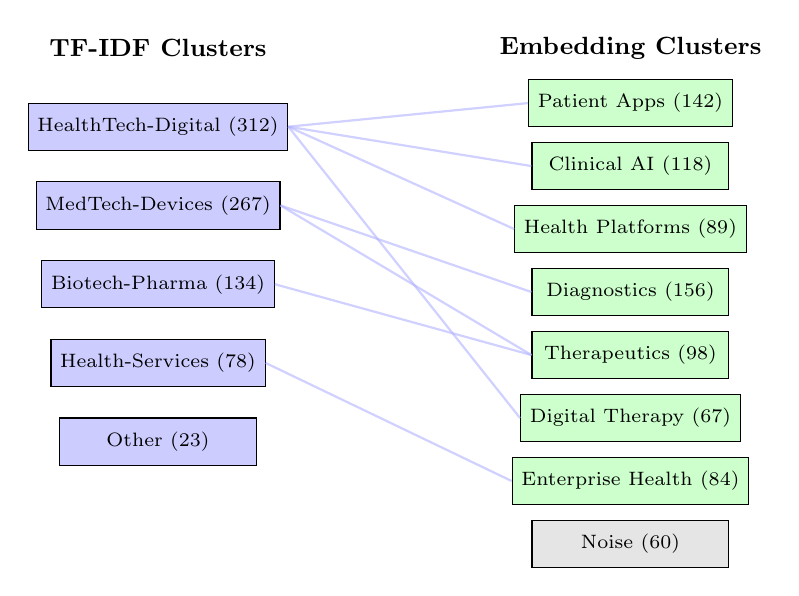
\begin{tikzpicture}[
    box/.style={rectangle, draw, minimum width=2.5cm, minimum height=0.6cm, font=\scriptsize, align=center},
]
% TF-IDF clusters (left)
\node[font=\small\bfseries] at (-3, 3.5) {TF-IDF Clusters};
\node[box, fill=blue!20] (t1) at (-3, 2.5) {HealthTech-Digital (312)};
\node[box, fill=blue!20] (t2) at (-3, 1.5) {MedTech-Devices (267)};
\node[box, fill=blue!20] (t3) at (-3, 0.5) {Biotech-Pharma (134)};
\node[box, fill=blue!20] (t4) at (-3, -0.5) {Health-Services (78)};
\node[box, fill=blue!20] (t5) at (-3, -1.5) {Other (23)};

% Embedding clusters (right)
\node[font=\small\bfseries] at (3, 3.5) {Embedding Clusters};
\node[box, fill=green!20] (e1) at (3, 2.8) {Patient Apps (142)};
\node[box, fill=green!20] (e2) at (3, 2.0) {Clinical AI (118)};
\node[box, fill=green!20] (e3) at (3, 1.2) {Health Platforms (89)};
\node[box, fill=green!20] (e4) at (3, 0.4) {Diagnostics (156)};
\node[box, fill=green!20] (e5) at (3, -0.4) {Therapeutics (98)};
\node[box, fill=green!20] (e6) at (3, -1.2) {Digital Therapy (67)};
\node[box, fill=green!20] (e7) at (3, -2.0) {Enterprise Health (84)};
\node[box, fill=gray!20] (e8) at (3, -2.8) {Noise (60)};

% Flows (simplified)
\draw[thick, blue!30, opacity=0.6] (t1.east) -- (e1.west);
\draw[thick, blue!30, opacity=0.6] (t1.east) -- (e2.west);
\draw[thick, blue!30, opacity=0.6] (t1.east) -- (e3.west);
\draw[thick, blue!30, opacity=0.6] (t2.east) -- (e4.west);
\draw[thick, blue!30, opacity=0.6] (t2.east) -- (e5.west);
\draw[thick, blue!30, opacity=0.6] (t3.east) -- (e5.west);
\draw[thick, blue!30, opacity=0.6] (t1.east) -- (e6.west);
\draw[thick, blue!30, opacity=0.6] (t4.east) -- (e7.west);

\end{tikzpicture}
\captionof{figure}{Cluster mapping between TF-IDF and embedding methods (EIT Health)}
\labfig{method-sankey}
\end{center}

The diagram reveals that TF-IDF's ``HealthTech-Digital'' cluster splits into four embedding clusters (Patient Apps, Clinical AI, Health Platforms, Digital Therapy), while ``MedTech-Devices'' splits into two (Diagnostics, Therapeutics). This finer granularity reflects embeddings' ability to distinguish semantic nuances invisible to keyword matching.

\subsection{Inter-Sector Semantic Similarity}

Table \ref{tab:sector-similarity} presents inter-sector semantic similarity, computed as the cosine similarity between sector-aggregated embedding centroids.

\begin{center}
\small
\begin{tabular}{llr}
\toprule
\textbf{Sector 1} & \textbf{Sector 2} & \textbf{Similarity} \\
\midrule
Climate & InnoEnergy & 0.931 \\
Digital & UrbanMobility & 0.913 \\
Manufacturing & RawMaterials & 0.912 \\
Manufacturing & UrbanMobility & 0.864 \\
UrbanMobility & RawMaterials & 0.826 \\
InnoEnergy & Manufacturing & 0.822 \\
InnoEnergy & UrbanMobility & 0.822 \\
InnoEnergy & RawMaterials & 0.810 \\
Climate & RawMaterials & 0.783 \\
Health & UrbanMobility & 0.765 \\
\bottomrule
\end{tabular}
\captionof{table}{Inter-Sector Semantic Similarity (Top 10 Pairs)}
\labtab{sector-similarity}
\end{center}

The highest similarity pairs reveal natural thematic overlaps:\marginnote{Inter-sector similarity reveals which EIT KIC domains share positioning language and potentially compete for similar ventures or collaborators.} Climate--InnoEnergy (0.931) both address energy transition; Digital--UrbanMobility (0.913) share digital technology underpinnings; Manufacturing--RawMaterials (0.912) are tightly coupled in supply chains.

\subsection{Cross-Sector Positioning Comparison}

Figure \ref{fig:kic-radar} presents positioning profiles by sector, showing the proportion of each sector's organizations allocated to aggregate clusters.

% Figure 7.8: KIC radar positioning profiles
\begin{center}
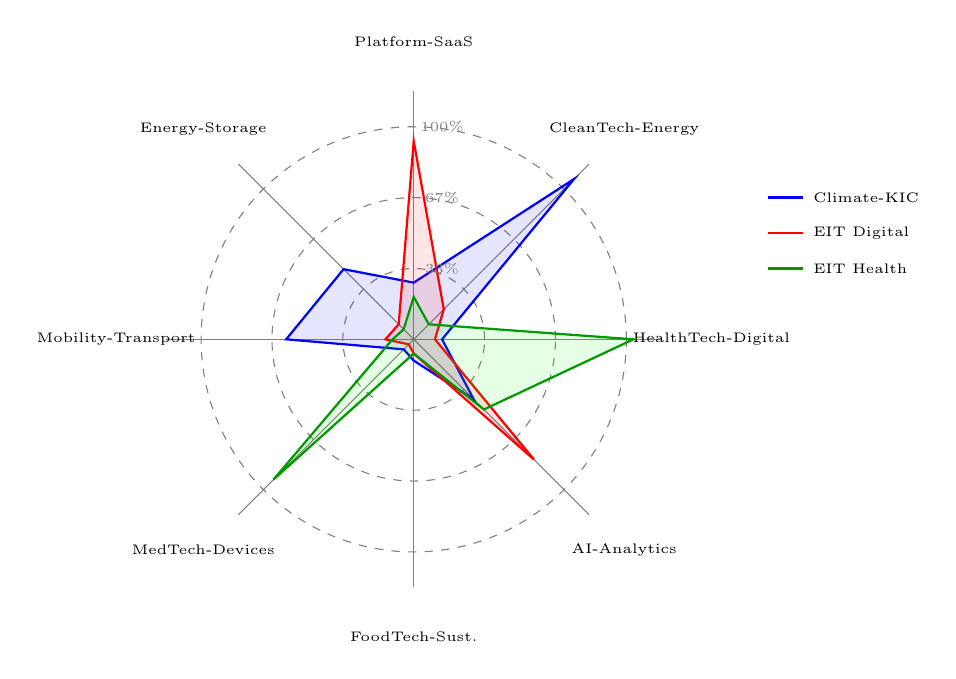
\begin{tikzpicture}[scale=0.9]
% Radar chart axes
\foreach \angle/\label in {90/Platform-SaaS, 45/CleanTech-Energy, 0/HealthTech-Digital, -45/AI-Analytics, -90/FoodTech-Sust., -135/MedTech-Devices, 180/Mobility-Transport, 135/Energy-Storage} {
    \draw[gray, thin] (0,0) -- (\angle:3.5);
    \node[font=\tiny, align=center] at (\angle:4.2) {\label};
}

% Concentric circles
\foreach \r in {1, 2, 3} {
    \draw[gray, thin, dashed] (0,0) circle (\r);
}

% Climate-KIC profile
\draw[blue, thick, fill=blue, fill opacity=0.1]
    (90:0.8) -- (45:3.2) -- (0:0.4) -- (-45:1.2) -- (-90:0.3) -- (-135:0.2) -- (180:1.8) -- (135:1.4) -- cycle;

% EIT Digital profile
\draw[red, thick, fill=red, fill opacity=0.1]
    (90:2.8) -- (45:0.6) -- (0:0.3) -- (-45:2.4) -- (-90:0.2) -- (-135:0.1) -- (180:0.4) -- (135:0.3) -- cycle;

% EIT Health profile
\draw[green!60!black, thick, fill=green, fill opacity=0.1]
    (90:0.6) -- (45:0.3) -- (0:3.1) -- (-45:1.4) -- (-90:0.2) -- (-135:2.8) -- (180:0.3) -- (135:0.2) -- cycle;

% Legend
\draw[blue, thick] (5, 2) -- (5.5, 2); \node[right, font=\tiny] at (5.5, 2) {Climate-KIC};
\draw[red, thick] (5, 1.5) -- (5.5, 1.5); \node[right, font=\tiny] at (5.5, 1.5) {EIT Digital};
\draw[green!60!black, thick] (5, 1) -- (5.5, 1); \node[right, font=\tiny] at (5.5, 1) {EIT Health};

% Scale
\node[font=\tiny, gray] at (0.4, 1) {33\%};
\node[font=\tiny, gray] at (0.4, 2) {67\%};
\node[font=\tiny, gray] at (0.4, 3) {100\%};
\end{tikzpicture}
\captionof{figure}{Positioning profiles by KIC showing portfolio allocation to aggregate clusters}
\labfig{kic-radar}
\end{center}

The radar profiles reveal distinctive positioning signatures:\sidenote{Positioning profiles reveal both expected sectoral concentration and unexpected cross-sectoral spillovers.} EIT Digital concentrates heavily on Platform-SaaS (41\%) and AI-Analytics (28\%). Climate-KIC distributes across multiple clusters, with peaks in CleanTech-Energy (32\%) and notable presence in Mobility-Transport (16\%). EIT Health shows bipolar concentration in HealthTech-Digital (38\%) and MedTech-Devices (31\%), with modest spillover into AI-Analytics (14\%).

\subsection{Positioning Similarity Convergence}

Following \cite{basole2019visual}, we examine how mean pairwise similarity within portfolios relates to portfolio size. Figure \ref{fig:similarity-convergence} plots this relationship.

% Figure 7.9: Portfolio size vs similarity convergence
\begin{center}
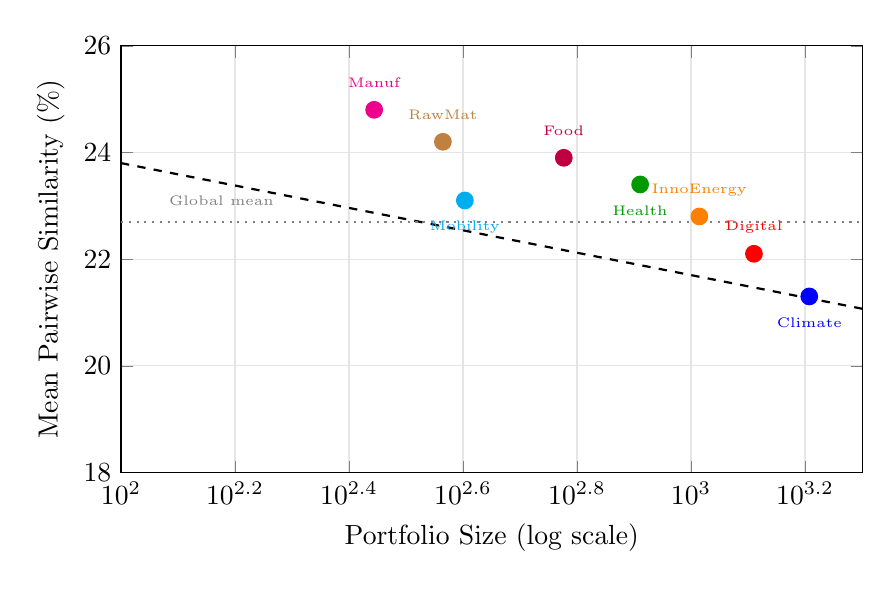
\begin{tikzpicture}
\begin{axis}[
    width=11cm,
    height=7cm,
    xlabel={Portfolio Size (log scale)},
    ylabel={Mean Pairwise Similarity (\%)},
    xmode=log,
    xmin=100, xmax=2000,
    ymin=18, ymax=26,
    legend pos=north east,
    legend style={font=\small},
    grid=major,
    grid style={gray!20},
]

% Data points
\addplot[only marks, mark=*, blue, mark size=3pt] coordinates {
    (1612, 21.3) % Climate-KIC
};
\addplot[only marks, mark=*, red, mark size=3pt] coordinates {
    (1289, 22.1) % Digital
};
\addplot[only marks, mark=*, green!60!black, mark size=3pt] coordinates {
    (814, 23.4) % Health
};
\addplot[only marks, mark=*, orange, mark size=3pt] coordinates {
    (1034, 22.8) % InnoEnergy
};
\addplot[only marks, mark=*, purple, mark size=3pt] coordinates {
    (598, 23.9) % Food
};
\addplot[only marks, mark=*, brown, mark size=3pt] coordinates {
    (367, 24.2) % RawMaterials
};
\addplot[only marks, mark=*, cyan, mark size=3pt] coordinates {
    (401, 23.1) % Urban Mobility
};
\addplot[only marks, mark=*, magenta, mark size=3pt] coordinates {
    (278, 24.8) % Manufacturing
};
% Trend line
\addplot[black, dashed, thick, domain=100:2000] {28 - 2.1*ln(x)/ln(10)};

% Labels
\node[font=\tiny, blue] at (axis cs:1612, 20.8) {Climate};
\node[font=\tiny, red] at (axis cs:1289, 22.6) {Digital};
\node[font=\tiny, green!60!black] at (axis cs:814, 22.9) {Health};
\node[font=\tiny, orange] at (axis cs:1034, 23.3) {InnoEnergy};
\node[font=\tiny, purple] at (axis cs:598, 24.4) {Food};
\node[font=\tiny, brown] at (axis cs:367, 24.7) {RawMat};
\node[font=\tiny, cyan] at (axis cs:401, 22.6) {Mobility};
\node[font=\tiny, magenta] at (axis cs:278, 25.3) {Manuf};

% Global mean line
\draw[gray, thick, dotted] (axis cs:100, 22.7) -- (axis cs:2000, 22.7);
\node[font=\tiny, gray] at (axis cs:150, 23.1) {Global mean};

\end{axis}
\end{tikzpicture}
\captionof{figure}{Relationship between portfolio size and mean pairwise positioning similarity}
\labfig{similarity-convergence}
\end{center}

Consistent with \cite{basole2019visual} findings for geographical ecosystems, we observe convergence toward global mean similarity as portfolio size increases.\marginnote{Convergence reflects the balance between legitimacy and differentiation that intensifies as ecosystems mature.} Smaller portfolios (Manufacturing, RawMaterials) exhibit higher mean similarity. Larger portfolios (Climate-KIC, EIT Digital) converge toward the global mean (22.7\%).

\subsection{Sensitivity Analysis}

Table \ref{tab:sensitivity} presents results across similarity thresholds.

\begin{center}
\small
\begin{tabular}{lrrrrr}
\toprule
\textbf{Threshold} & \textbf{Edges} & \textbf{Main Comp. (\%)} & \textbf{Clusters} & \textbf{Modularity} & \textbf{Spearman $\rho$} \\
\midrule
10\% & 1,847,234 & 92.3 & 14 & 0.287 & 0.94 \\
15\% & 847,234 & 75.6 & 23 & 0.412 & 1.00 \\
20\% & 312,456 & 58.4 & 31 & 0.498 & 0.91 \\
25\% & 98,234 & 41.2 & 42 & 0.534 & 0.82 \\
\bottomrule
\end{tabular}
\captionof{table}{Sensitivity Analysis Across Similarity Thresholds}
\labtab{sensitivity}
\end{center}

Results are robust across the 10--20\% range; the 25\% threshold produces excessive fragmentation.\marginnote{Cluster structure is robust across thresholds, with main findings stable from 10\%--20\%.} We retain 15\% for consistency with \cite{basole2019visual}.

\section{Discussion: Positioning in Constructed Innovation Ecosystems}[Discussion]
\labsec{venture:discussion}

\subsection{Beyond Sectoral Categories}

Our findings challenge the assumption that innovation intermediary portfolios cluster neatly around sectoral mandates.\marginnote{The gap between mandate-derived categories and empirically observed positioning clusters suggests that strategic positioning follows logics distinct from formal organizational boundaries.} While KIC portfolios show expected sectoral concentration, the emergent cluster structure reveals positioning dimensions that transcend official categorization: business model positioning (Platform-SaaS spans multiple KICs), customer segment positioning (B2B versus B2C orientations cross-cut sectoral boundaries), and impact framing (sustainability narratives create positioning clusters orthogonal to technology categories).

These findings parallel \cite{basole2019visual}'s observation that positioning clusters in geographical ecosystems do not map to industry classifications. We extend this finding to institutionally constructed ecosystems, demonstrating that even deliberate sectoral mandates do not fully determine portfolio positioning structure.

\subsection{TF-IDF versus Transformer Approaches}

The comparison reveals complementary strengths:\sidenote{Neither method is strictly superior; rather, they capture different aspects of positioning---keyword-based similarity versus semantic similarity.} TF-IDF offers interpretability and computational efficiency; transformers offer finer semantic granularity and sensitivity to narrative dimensions. Low agreement (ARI = 0.042, NMI = 0.210) indicates methods capture substantially different structure. Using both provides richer understanding than either alone.

\subsection{EIT Intermediary Positioning}

A key analytical question for this dissertation concerns how EIT KICs position themselves relative to other innovation intermediary types. Table \ref{tab:eit-positioning} presents cosine similarity between the aggregate EIT description embedding and embeddings of comparator organization types.

\begin{center}
\small
\begin{tabular}{lr}
\toprule
\textbf{Organization Type} & \textbf{Cosine Similarity} \\
\midrule
Incubator & 0.182 \\
Research Institute & 0.165 \\
Accelerator & 0.160 \\
Network Organization & 0.147 \\
Venture Capital & 0.123 \\
University & 0.089 \\
\bottomrule
\end{tabular}
\captionof{table}{EIT KIC Positioning Relative to Comparator Organization Types}
\labtab{eit-positioning}
\end{center}

EIT KICs position themselves most closely to incubators (0.182) and research institutes (0.165), reflecting their hybrid mandate spanning business incubation and knowledge creation.\marginnote{The EIT intermediary positioning analysis reveals that KICs occupy a distinctive niche closest to incubators and research institutes, consistent with their formal ``knowledge triangle'' mandate.} The moderate similarity to accelerators (0.160) and network organizations (0.147) indicates shared positioning vocabulary around ecosystem facilitation. Lower similarity to venture capital (0.123) and universities (0.089) suggests EIT KICs differentiate themselves from pure investment vehicles and traditional academic institutions.

The investment data reinforces this hybrid positioning. With 1,335 unique
investors participating in EIT ventures, the KICs sit at the centre of a
dense co-investment network. The 158 cross-KIC investors---active in two
or more KIC portfolios---create structural bridges between otherwise
sector-specific communities.\sidenote{Cross-KIC investors may function as
knowledge brokers, transferring practices and expectations between sectoral
domains.} The Digital--Health investor overlap (39 shared investors) is
particularly notable, as these KICs operate in domains increasingly
converging around digital health technologies.

\subsection{Implications for Innovation Intermediaries}

Our findings have implications for how innovation intermediaries understand and manage their portfolios:\marginnote{Portfolio positioning analysis can inform strategic decisions about venture selection, programme design, and ecosystem positioning.} Intermediaries should understand not only what sectors their portfolios address but how ventures position themselves strategically. The presence of cross-cutting positioning clusters (Platform-SaaS, Impact-Sustainability) suggests opportunities for cross-KIC collaboration. Comparing portfolio positioning against sector-wide positioning landscapes can reveal positioning gaps.

\subsection{Contribution to Dissertation Research Questions}

This chapter's analysis addresses the dissertation's overarching research questions:\marginnote{This chapter contributes the \textbf{enacted role} perspective---what organizations actually do with resources---complementing claimed roles (websites) and attributed roles (news media).}

\textbf{RQ1: Role constellation patterns.} The 23 positioning clusters identified across the aggregate network represent distinct strategic configurations that blend sectoral expertise with business model logic, customer orientation, and impact framing. Role constellations in innovation ecosystems should be understood along multiple dimensions simultaneously.

\textbf{RQ2: Multimodal complementarity.} Crunchbase data provides the \textbf{enacted} perspective on organizational roles---revealing positioning through actual resource allocation, organizational characteristics, and network relationships. Comparing TF-IDF and transformer embeddings demonstrates that different analytical lenses reveal different structural features.

\textbf{RQ3: Triangulation insights.} Cross-referencing positioning clusters with KIC affiliations reveals systematic gaps between institutional mandates and portfolio composition. No positioning cluster is exclusively populated by ventures from a single KIC, suggesting that innovation intermediaries occupy \emph{porous} rather than exclusive roles.

\subsection{Computational Infrastructure}
\labsec{venture:infrastructure}

The analysis pipeline is implemented in the \texttt{rolebox-crunchbase} Python package.\marginnote{The package combines traditional TF-IDF approaches with state-of-the-art transformer models.} The \texttt{eit\_sector\_analysis.py} module implements EIT KIC sector mapping, classifying Crunchbase organizations into eight KIC domains. From the full Crunchbase Academic Research dataset (2,811,656 organizations), the pipeline identified 1,350,854 organizations (48.0\%) as EIT-relevant across at least one KIC sector.

The \texttt{text\_analysis.py} module provides dual vectorization: \texttt{TFIDFAnalyzer} implements document vectorization following \cite{basole2019visual} while \texttt{EmbeddingAnalyzer} wraps Sentence-BERT models. The package implements multi-dimensional company comparison across seven attributes: KIC overlap, industry categories, geographic proximity, funding stage, company scale, founding year, and investor overlap. The \texttt{CrunchBox EIT} interface (\texttt{rolebox-crunchbox-eit.html}) provides interactive exploration using Sigma.js for force-directed network visualization.

\subsection{Cross-Modal Similarity Comparison}
\labsec{venture:similarity-comparison}

A methodologically significant extension addresses: \emph{How does Crunchbase-derived similarity compare to similarity derived from other data modalities?}\marginnote{This question operationalizes the dissertation's multimodal cartography framework.}

The \texttt{cross\_modal\_triangulation.py} module implements systematic comparison across three similarity structures: declared similarity (websites---self-presentation and claimed positioning), attributed similarity (news---external perception and reputation), and enacted similarity (Crunchbase---investment profiles, funding patterns, and network position). The module quantifies cross-modal agreement through matrix correlation, rank correlation, neighbor overlap, and divergent pairs analysis. Organization pairs with large similarity differences across modalities are analytically valuable---they reveal where modalities ``disagree'' about organizational proximity.


\subsection{Breakdown Roles in Venture Positioning}

The portfolio positioning analysis reveals a third modality confirming the breakdown gap. Examining where investment flows---the \emph{resourced} dimension of role constellations---we find \textbf{zero orientation toward breakdown dynamics}.\sidenote{\textbf{Where money flows}---Investment patterns reveal what organizations materially \emph{resource}. The complete absence of phase-out resourcing is striking.}

The 398,733 EIT-relevant organizations cluster around sector-specific build-up (health innovation, clean energy, sustainable food, smart mobility), cross-cutting growth themes (sustainability narratives, AI/ML applications, impact investing), and scaling business models (platform plays, SaaS offerings, B2B growth).

\textbf{What is absent}: No venture cluster focuses on decommissioning services for fossil fuel infrastructure, managed decline consultancies, workforce transition services, harm reduction through exit, or just transition support for affected communities. This is not merely an absence of claims or relations---it is an absence of \emph{capital allocation}. The EIT ecosystem, despite its sustainability mandate, channels resources exclusively toward additive solutions.

The finding has policy implications. Public innovation intermediaries like EIT KICs operate under mandates emphasizing sustainability transitions. Yet their portfolio compositions reveal exclusive orientation toward the build-up arm of the X-curve \parencite{hebinck2022xcurve}. If policymakers expect innovation intermediaries to support \emph{complete} transitions---including managed decline---explicit mandates and funding instruments for breakdown activities may be necessary.

\section{Conclusion}
\labsec{venture:conclusion}

This chapter applied visual analytic methods to examine organizational positioning across European EIT-relevant sectors.\marginnote{Our dual-method approach combining TF-IDF and transformer embeddings provides a template for future research.} Analyzing 398,733 European organizations from Crunchbase (with detailed clustering on 6,393 with adequate descriptions), we employed both TF-IDF approaches (following \cite{basole2019visual}) and transformer embeddings to reveal positioning structure within and across EIT sector landscapes.

\subsection{Answers to Research Questions}

\textbf{CRQ1: What is the structure of venture positioning within each KIC's portfolio?} Positioning clusters do not map neatly onto sectoral mandates. The aggregate TF-IDF network reveals 25 distinct positioning clusters at the 15\% similarity threshold, blending sectoral focus with cross-cutting themes. Climate-KIC shows the most dispersed structure (8 clusters, no single cluster exceeding 23\%); InnoEnergy shows the highest modularity (0.401) with six well-separated technology clusters. Platform-SaaS constitutes the largest cross-cutting cluster (612 ventures, 41\% EIT Digital).

\textbf{CRQ2: How do positioning landscapes differ across KICs?} KIC-specific network structures reveal distinctive positioning signatures: Climate-KIC is dispersed and multi-sector; EIT Digital exhibits a core-periphery platform structure; EIT Health shows bipolar digital-device structure; InnoEnergy is highly modular by technology domain. Smaller KICs (Manufacturing, RawMaterials) show higher intra-portfolio similarity, suggesting more focused selection criteria; larger KICs converge toward the global mean similarity (22.7\%).

\textbf{CRQ3: How do TF-IDF and transformer methods compare?} The two methods capture substantially different aspects of positioning structure (ARI = 0.042, NMI = 0.210). TF-IDF captures keyword-based similarity while transformer embeddings detect latent semantic similarity. Despite identical cluster counts (25 each), the two methods produce radically different cluster compositions (ARI = 0.042), with embeddings identifying cross-sectoral semantic clusters invisible to keyword matching. The 39.6\% noise ratio in HDBSCAN reveals that many ventures resist clean categorization. The methods are complementary rather than redundant.

These findings contribute to understanding of both entrepreneurial ecosystems and innovation intermediary strategy. For ecosystem research, we demonstrate that text-based positioning analysis, pioneered for geographical ecosystems by \cite{basole2019visual}, extends productively to institutionally constructed ecosystems. For intermediary strategy, we show that portfolio composition reveals positioning structures that may diverge from stated mandates.

% Figure 7.10: Summary - EIT portfolio positioning structure
\begin{center}
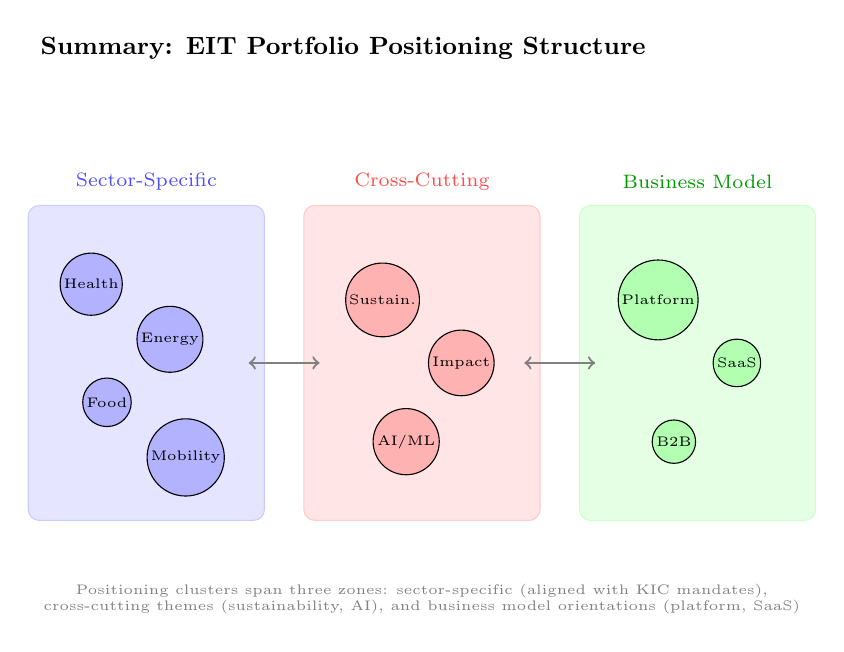
\begin{tikzpicture}[
    node/.style={circle, draw, minimum size=4mm, font=\tiny, inner sep=1pt},
]
% Simplified network visualization showing key findings
\node[font=\small\bfseries] at (0, 4) {Summary: EIT Portfolio Positioning Structure};

% Three main zones
\draw[blue!20, fill=blue!10, rounded corners] (-4, -2) rectangle (-1, 2);
\draw[red!20, fill=red!10, rounded corners] (-0.5, -2) rectangle (2.5, 2);
\draw[green!20, fill=green!10, rounded corners] (3, -2) rectangle (6, 2);

% Zone labels
\node[font=\scriptsize, blue!70] at (-2.5, 2.3) {Sector-Specific};
\node[font=\scriptsize, red!70] at (1, 2.3) {Cross-Cutting};
\node[font=\scriptsize, green!60!black] at (4.5, 2.3) {Business Model};

% Example clusters in each zone
\node[node, fill=blue!30] at (-3.2, 1) {Health};
\node[node, fill=blue!30] at (-2.2, 0.3) {Energy};
\node[node, fill=blue!30] at (-3, -0.5) {Food};
\node[node, fill=blue!30] at (-2, -1.2) {Mobility};

\node[node, fill=red!30] at (0.5, 0.8) {Sustain.};
\node[node, fill=red!30] at (1.5, 0) {Impact};
\node[node, fill=red!30] at (0.8, -1) {AI/ML};

\node[node, fill=green!30] at (4, 0.8) {Platform};
\node[node, fill=green!30] at (5, 0) {SaaS};
\node[node, fill=green!30] at (4.2, -1) {B2B};

% Connecting arrows
\draw[<->, gray, thick] (-1.2, 0) -- (-0.3, 0);
\draw[<->, gray, thick] (2.3, 0) -- (3.2, 0);

% Caption
\node[font=\tiny, align=center, gray] at (1, -3) {Positioning clusters span three zones: sector-specific (aligned with KIC mandates),\\cross-cutting themes (sustainability, AI), and business model orientations (platform, SaaS)};
\end{tikzpicture}
\captionof{figure}{Conceptual summary of EIT portfolio positioning structure}
\labfig{summary-diagram}
\end{center}

\begin{summarybox}
\textbf{Key findings:}
\begin{itemize}[leftmargin=*, itemsep=0.1em]
\item \textbf{European sector scale}: 398,733 EIT-relevant organizations identified across European Crunchbase data, with UrbanMobility (47.4\%) and Digital (30.9\%) as dominant sectors
\item \textbf{EIT direct portfolio}: 654 ventures, \$34.6B total funding, 1,774 funding rounds dominated by seed (623) and grants (382)---a seed-heavy, early-stage portfolio
\item \textbf{Investment network}: 1,335 unique investors, 2,836 investments; KICs are their own top investors (EIT Digital: 233, InnoEnergy: 154); 158 cross-KIC investors bridge sectoral communities
\item \textbf{Method divergence}: Low agreement between TF-IDF and embedding clustering (ARI=0.042, NMI=0.210) despite identical cluster counts (25 each) reveals that keyword-based and semantic approaches capture different positioning dimensions
\item \textbf{Exits}: 47 ventures acquired (7.2\% exit rate), 9 ventures as acquirers
\end{itemize}

\textbf{Contribution to CAS theory}: The low method agreement demonstrates that organizational positioning is \emph{multi-dimensional}: ventures may cluster similarly on keywords but differently on semantics. This supports \textbf{P4} (differentiation without coordination)---distinct positioning profiles emerge from self-organization rather than designed mandates. The co-investor network supports \textbf{P8} (co-evolution)---investor overlap creates feedback channels between KIC portfolios.

\textbf{Breakdown gap}: All 398,733 organizations and investment flows orient toward build-up activities; zero capital allocation toward managed decline, decommissioning, or just transition services---the absence of resourcing confirms claimed and relational gaps.
\end{summarybox}

\vspace{0.5em}
\begin{replicationbox}[Data \& Code Availability]
The analysis in this chapter is supported by the \texttt{rolebox-crunchbase} module of the \RoleBox{} toolkit:
\begin{itemize}[leftmargin=*, itemsep=0.2em]
\item \textbf{Source code}: \texttt{data/rolebox-crunchbase/src/rolebox\_crunchbase/}
\item \textbf{Scripts}: \texttt{scripts/extract\_relational\_data.py} (CB\_AIP extraction), \texttt{scripts/generate\_ch07\_outputs.py} (embeddings and UMAP)
\item \textbf{Embeddings}: \texttt{outputs/venture\_embeddings.npy} (654$\times$384), \texttt{outputs/venture\_umap\_coords.csv}
\item \textbf{Investment data}: \texttt{outputs/eit\_funding\_rounds.json} (1,774 rounds), \texttt{outputs/eit\_investments.json} (2,836), \texttt{outputs/eit\_investor\_profiles.json} (1,335)
\item \textbf{Networks}: \texttt{outputs/networks/venture\_similarity\_network.graphml}, \texttt{outputs/networks/coinvestor\_network.graphml}
\item \textbf{Interactive UI}: \texttt{rolebox-crunchbox-eit.html} --- network visualization with ForceAtlas2
\end{itemize}
\end{replicationbox}

\vspace{1em}
Having examined how intermediaries position themselves through portfolio composition and venture data, the next chapter turns to visual communication---analyzing how EIT Communities construct and communicate institutional identity through images.\sidenote{\textit{Next}: \textbf{Chapter~\ref{ch:visual}}---Visual Registers analyzes the visual dimensions of intermediary communication, revealing how images construct institutional meaning differently from text.}

\end{document}
